\documentclass[]{book}
\usepackage{lmodern}
\usepackage{amssymb,amsmath}
\usepackage{ifxetex,ifluatex}
\usepackage{fixltx2e} % provides \textsubscript
\ifnum 0\ifxetex 1\fi\ifluatex 1\fi=0 % if pdftex
  \usepackage[T1]{fontenc}
  \usepackage[utf8]{inputenc}
\else % if luatex or xelatex
  \ifxetex
    \usepackage{mathspec}
  \else
    \usepackage{fontspec}
  \fi
  \defaultfontfeatures{Ligatures=TeX,Scale=MatchLowercase}
  \newcommand{\euro}{€}
\fi
% use upquote if available, for straight quotes in verbatim environments
\IfFileExists{upquote.sty}{\usepackage{upquote}}{}
% use microtype if available
\IfFileExists{microtype.sty}{%
\usepackage{microtype}
\UseMicrotypeSet[protrusion]{basicmath} % disable protrusion for tt fonts
}{}
\usepackage[margin=1in]{geometry}
\usepackage{hyperref}
\PassOptionsToPackage{usenames,dvipsnames}{color} % color is loaded by hyperref
\hypersetup{unicode=true,
            pdftitle={Solutions to Time Series Analysis: with Applications in R},
            pdfauthor={Johan Larsson},
            pdfborder={0 0 0},
            breaklinks=true}
\urlstyle{same}  % don't use monospace font for urls
\usepackage{color}
\usepackage{fancyvrb}
\newcommand{\VerbBar}{|}
\newcommand{\VERB}{\Verb[commandchars=\\\{\}]}
\DefineVerbatimEnvironment{Highlighting}{Verbatim}{commandchars=\\\{\}}
% Add ',fontsize=\small' for more characters per line
\usepackage{framed}
\definecolor{shadecolor}{RGB}{248,248,248}
\newenvironment{Shaded}{\begin{snugshade}}{\end{snugshade}}
\newcommand{\KeywordTok}[1]{\textcolor[rgb]{0.13,0.29,0.53}{\textbf{{#1}}}}
\newcommand{\DataTypeTok}[1]{\textcolor[rgb]{0.13,0.29,0.53}{{#1}}}
\newcommand{\DecValTok}[1]{\textcolor[rgb]{0.00,0.00,0.81}{{#1}}}
\newcommand{\BaseNTok}[1]{\textcolor[rgb]{0.00,0.00,0.81}{{#1}}}
\newcommand{\FloatTok}[1]{\textcolor[rgb]{0.00,0.00,0.81}{{#1}}}
\newcommand{\ConstantTok}[1]{\textcolor[rgb]{0.00,0.00,0.00}{{#1}}}
\newcommand{\CharTok}[1]{\textcolor[rgb]{0.31,0.60,0.02}{{#1}}}
\newcommand{\SpecialCharTok}[1]{\textcolor[rgb]{0.00,0.00,0.00}{{#1}}}
\newcommand{\StringTok}[1]{\textcolor[rgb]{0.31,0.60,0.02}{{#1}}}
\newcommand{\VerbatimStringTok}[1]{\textcolor[rgb]{0.31,0.60,0.02}{{#1}}}
\newcommand{\SpecialStringTok}[1]{\textcolor[rgb]{0.31,0.60,0.02}{{#1}}}
\newcommand{\ImportTok}[1]{{#1}}
\newcommand{\CommentTok}[1]{\textcolor[rgb]{0.56,0.35,0.01}{\textit{{#1}}}}
\newcommand{\DocumentationTok}[1]{\textcolor[rgb]{0.56,0.35,0.01}{\textbf{\textit{{#1}}}}}
\newcommand{\AnnotationTok}[1]{\textcolor[rgb]{0.56,0.35,0.01}{\textbf{\textit{{#1}}}}}
\newcommand{\CommentVarTok}[1]{\textcolor[rgb]{0.56,0.35,0.01}{\textbf{\textit{{#1}}}}}
\newcommand{\OtherTok}[1]{\textcolor[rgb]{0.56,0.35,0.01}{{#1}}}
\newcommand{\FunctionTok}[1]{\textcolor[rgb]{0.00,0.00,0.00}{{#1}}}
\newcommand{\VariableTok}[1]{\textcolor[rgb]{0.00,0.00,0.00}{{#1}}}
\newcommand{\ControlFlowTok}[1]{\textcolor[rgb]{0.13,0.29,0.53}{\textbf{{#1}}}}
\newcommand{\OperatorTok}[1]{\textcolor[rgb]{0.81,0.36,0.00}{\textbf{{#1}}}}
\newcommand{\BuiltInTok}[1]{{#1}}
\newcommand{\ExtensionTok}[1]{{#1}}
\newcommand{\PreprocessorTok}[1]{\textcolor[rgb]{0.56,0.35,0.01}{\textit{{#1}}}}
\newcommand{\AttributeTok}[1]{\textcolor[rgb]{0.77,0.63,0.00}{{#1}}}
\newcommand{\RegionMarkerTok}[1]{{#1}}
\newcommand{\InformationTok}[1]{\textcolor[rgb]{0.56,0.35,0.01}{\textbf{\textit{{#1}}}}}
\newcommand{\WarningTok}[1]{\textcolor[rgb]{0.56,0.35,0.01}{\textbf{\textit{{#1}}}}}
\newcommand{\AlertTok}[1]{\textcolor[rgb]{0.94,0.16,0.16}{{#1}}}
\newcommand{\ErrorTok}[1]{\textcolor[rgb]{0.64,0.00,0.00}{\textbf{{#1}}}}
\newcommand{\NormalTok}[1]{{#1}}
\usepackage{longtable,booktabs}
\usepackage{graphicx,grffile}
\makeatletter
\def\maxwidth{\ifdim\Gin@nat@width>\linewidth\linewidth\else\Gin@nat@width\fi}
\def\maxheight{\ifdim\Gin@nat@height>\textheight\textheight\else\Gin@nat@height\fi}
\makeatother
% Scale images if necessary, so that they will not overflow the page
% margins by default, and it is still possible to overwrite the defaults
% using explicit options in \includegraphics[width, height, ...]{}
\setkeys{Gin}{width=\maxwidth,height=\maxheight,keepaspectratio}
\setlength{\parindent}{0pt}
\setlength{\parskip}{6pt plus 2pt minus 1pt}
\setlength{\emergencystretch}{3em}  % prevent overfull lines
\providecommand{\tightlist}{%
  \setlength{\itemsep}{0pt}\setlength{\parskip}{0pt}}
\setcounter{secnumdepth}{5}

%%% Use protect on footnotes to avoid problems with footnotes in titles
\let\rmarkdownfootnote\footnote%
\def\footnote{\protect\rmarkdownfootnote}

%%% Change title format to be more compact
\usepackage{titling}

% Create subtitle command for use in maketitle
\newcommand{\subtitle}[1]{
  \posttitle{
    \begin{center}\large#1\end{center}
    }
}

\setlength{\droptitle}{-2em}
  \title{Solutions to Time Series Analysis: with Applications in R}
  \pretitle{\vspace{\droptitle}\centering\huge}
  \posttitle{\par}
  \author{Johan Larsson}
  \preauthor{\centering\large\emph}
  \postauthor{\par}
  \predate{\centering\large\emph}
  \postdate{\par}
  \date{2017-04-04}


% Redefines (sub)paragraphs to behave more like sections
\ifx\paragraph\undefined\else
\let\oldparagraph\paragraph
\renewcommand{\paragraph}[1]{\oldparagraph{#1}\mbox{}}
\fi
\ifx\subparagraph\undefined\else
\let\oldsubparagraph\subparagraph
\renewcommand{\subparagraph}[1]{\oldsubparagraph{#1}\mbox{}}
\fi


\begin{document}
\maketitle

{
\setcounter{tocdepth}{1}
\tableofcontents
}
\chapter*{Preface}\label{preface}
\addcontentsline{toc}{chapter}{Preface}

This book contains solutions to the problems in the book \emph{Time
Series Analysis: with Applications in R}, third edition, by Cryer and
Chan. It is provided as a github repository so that anybody may
contribute to its development. Unlike the book, the solutions here use
lattice graphics when possible instead of base graphics.

\chapter{Introduction}\label{introduction}

\section{Larain}\label{larain}

\begin{quote}
Use software to produce the time series plot shown in Exhibit 1.2, on
page 2. The data are in the file named larain.
\end{quote}

\begin{Shaded}
\begin{Highlighting}[]
\KeywordTok{library}\NormalTok{(TSA)}
\KeywordTok{library}\NormalTok{(latticeExtra)}

\KeywordTok{data}\NormalTok{(larain, }\DataTypeTok{package =} \StringTok{"TSA"}\NormalTok{)}
\end{Highlighting}
\end{Shaded}

\begin{Shaded}
\begin{Highlighting}[]
\KeywordTok{xyplot}\NormalTok{(larain, }\DataTypeTok{ylab =} \StringTok{"Inches"}\NormalTok{, }\DataTypeTok{xlab =} \StringTok{"Year"}\NormalTok{, }\DataTypeTok{type =} \StringTok{"o"}\NormalTok{)}
\end{Highlighting}
\end{Shaded}

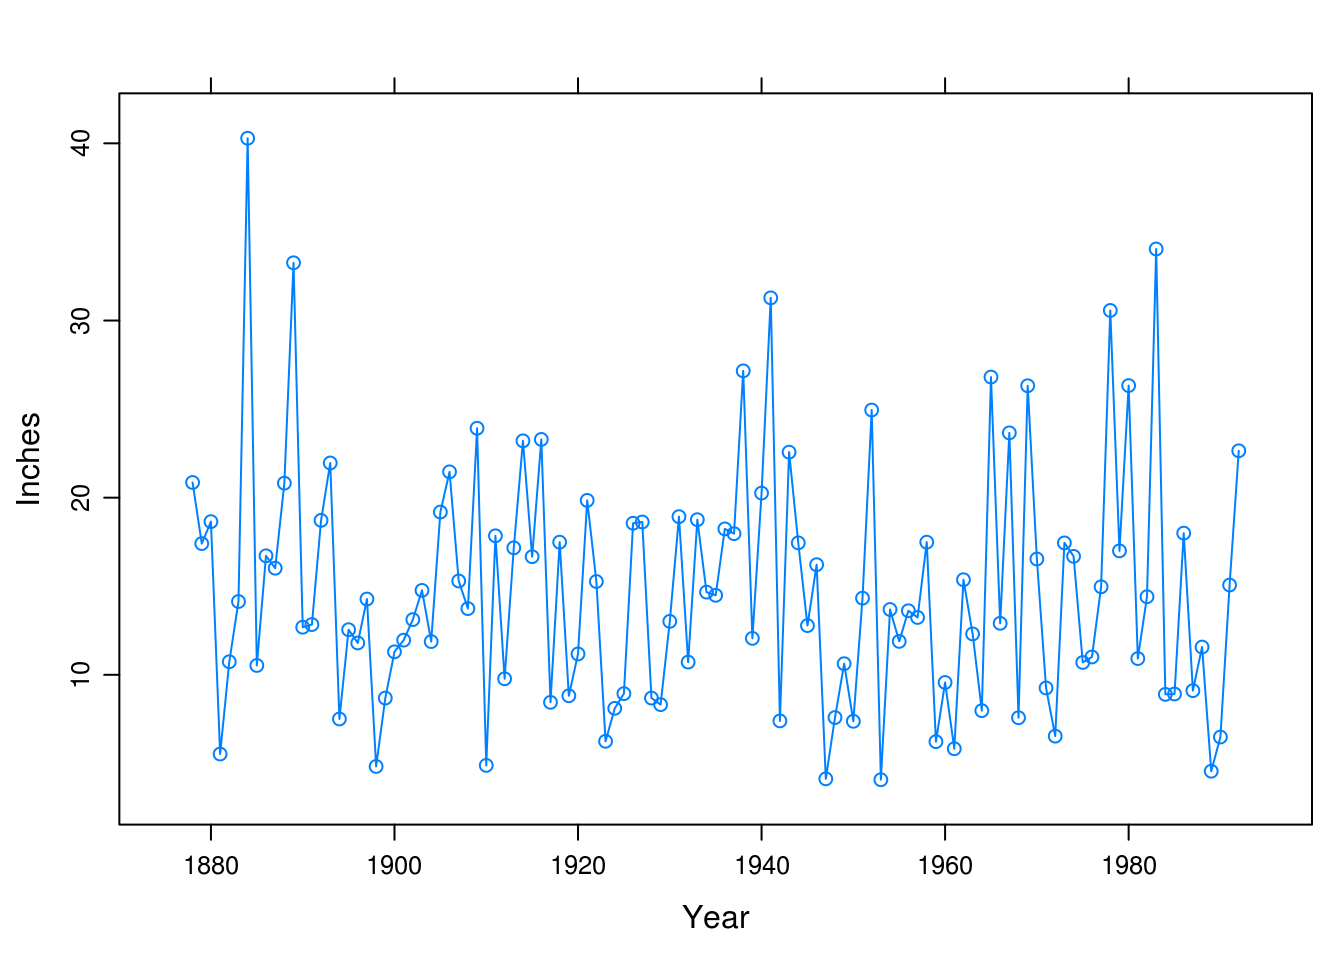
\includegraphics{TSAsolutions_files/figure-latex/unnamed-chunk-1-1.pdf}

\section{Colors}\label{colors}

\begin{quote}
Produce the time series plot displayed in Exhibit 1.3, on page 3. The
data file is named color.
\end{quote}

\begin{Shaded}
\begin{Highlighting}[]
\KeywordTok{data}\NormalTok{(color)}
\KeywordTok{xyplot}\NormalTok{(color, }\DataTypeTok{ylab =} \StringTok{"Color property"}\NormalTok{, }\DataTypeTok{xlab =} \StringTok{"Batch"}\NormalTok{, }\DataTypeTok{type =} \StringTok{"o"}\NormalTok{)}
\end{Highlighting}
\end{Shaded}

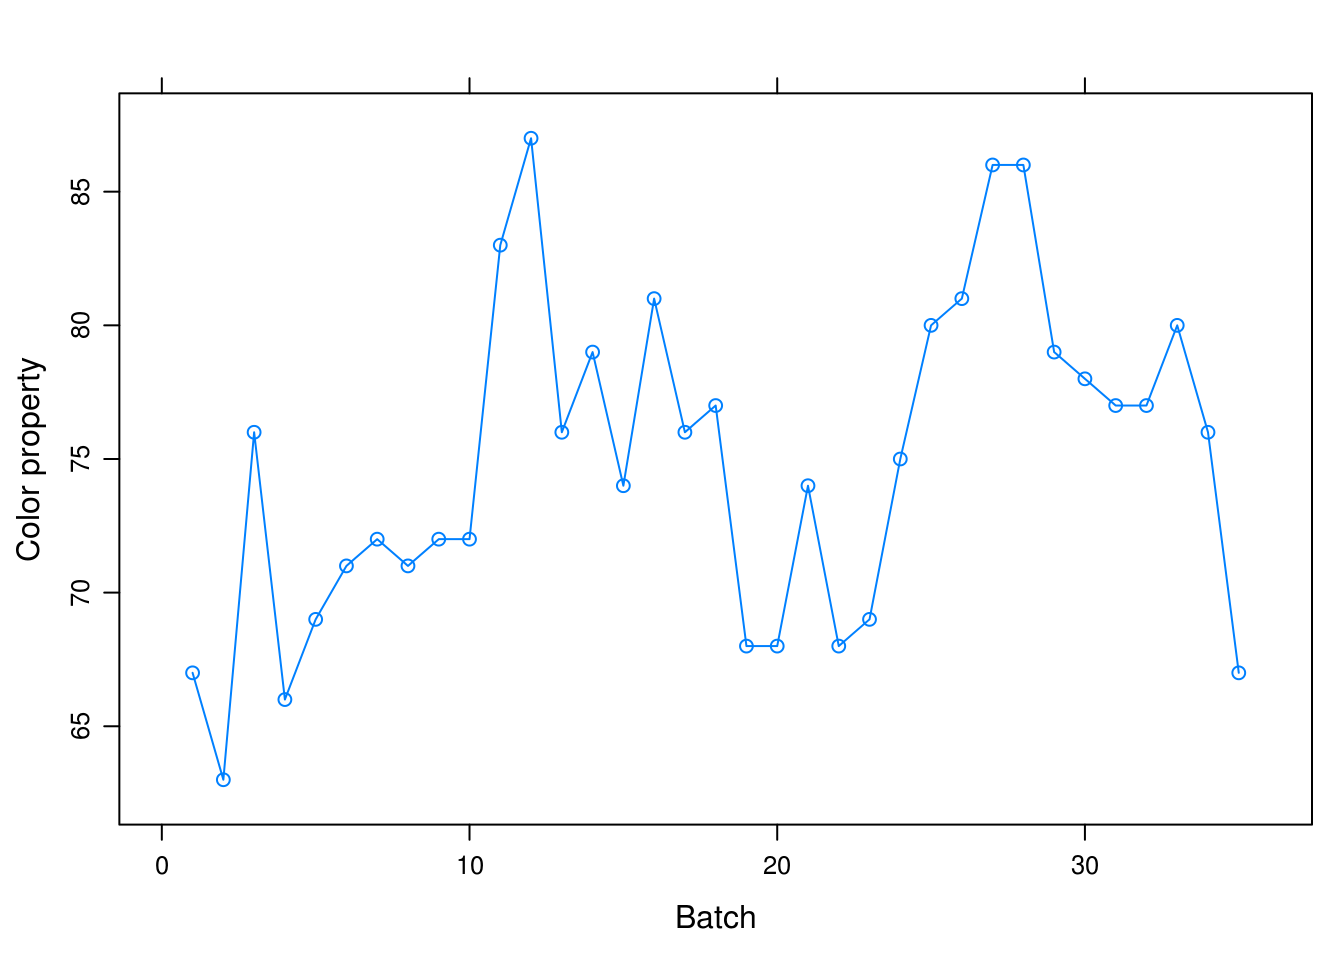
\includegraphics{TSAsolutions_files/figure-latex/unnamed-chunk-2-1.pdf}

\section{Random, normal time series}\label{random-normal-time-series}

\begin{quote}
Simulate a completely random process of length 48 with independent,
normal values. Plot the time series plot. Does it look ``random''?
Repeat this exercise several times with a new simulation each time.
\end{quote}

\begin{Shaded}
\begin{Highlighting}[]
\KeywordTok{xyplot}\NormalTok{(}\KeywordTok{as.ts}\NormalTok{(}\KeywordTok{rnorm}\NormalTok{(}\DecValTok{48}\NormalTok{)))}
\KeywordTok{xyplot}\NormalTok{(}\KeywordTok{as.ts}\NormalTok{(}\KeywordTok{rnorm}\NormalTok{(}\DecValTok{48}\NormalTok{)))}
\end{Highlighting}
\end{Shaded}

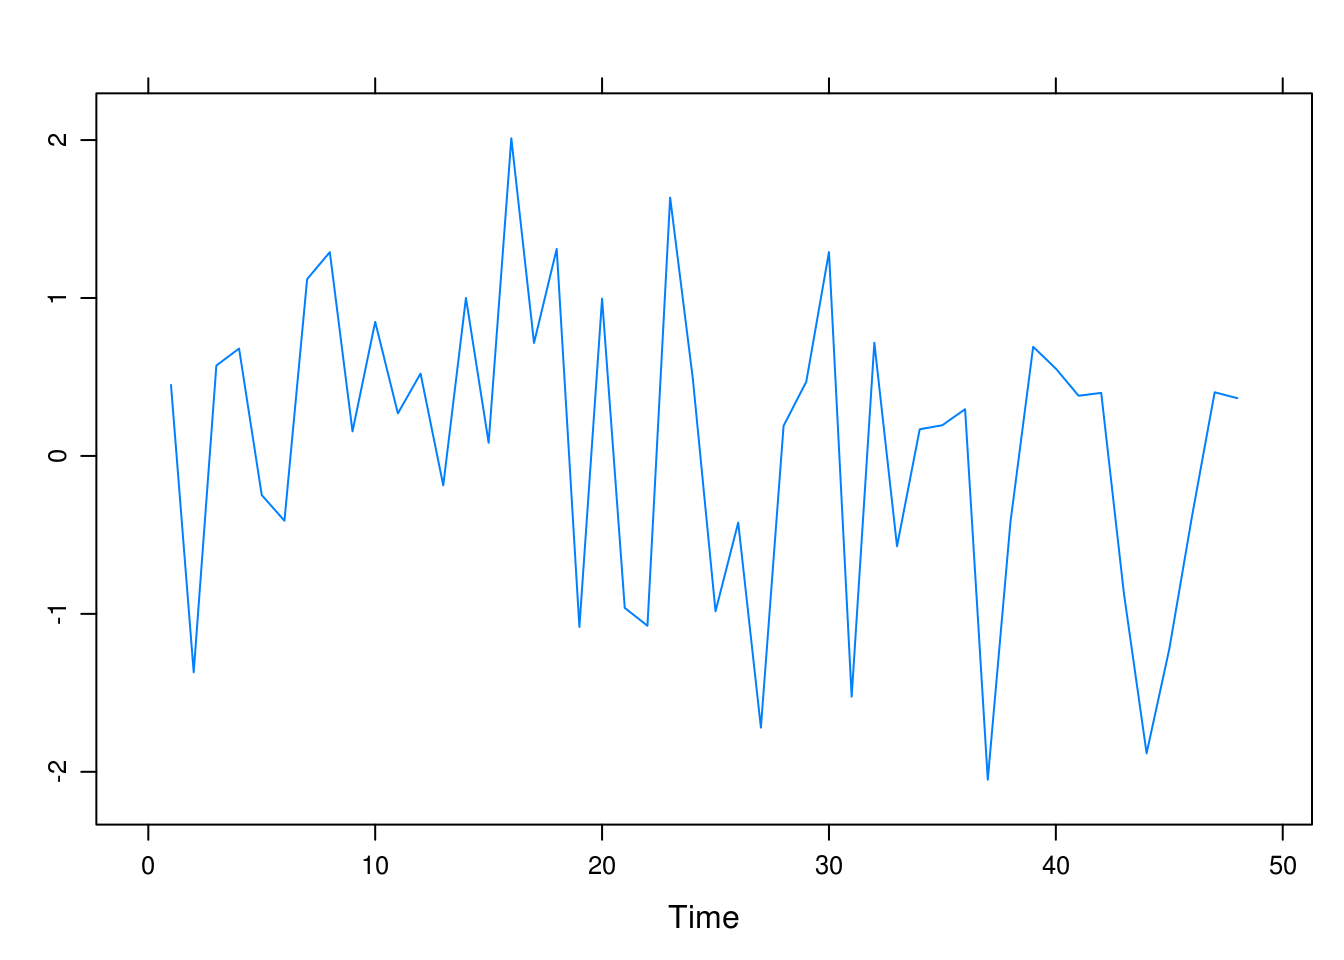
\includegraphics{TSAsolutions_files/figure-latex/unnamed-chunk-3-1.pdf}
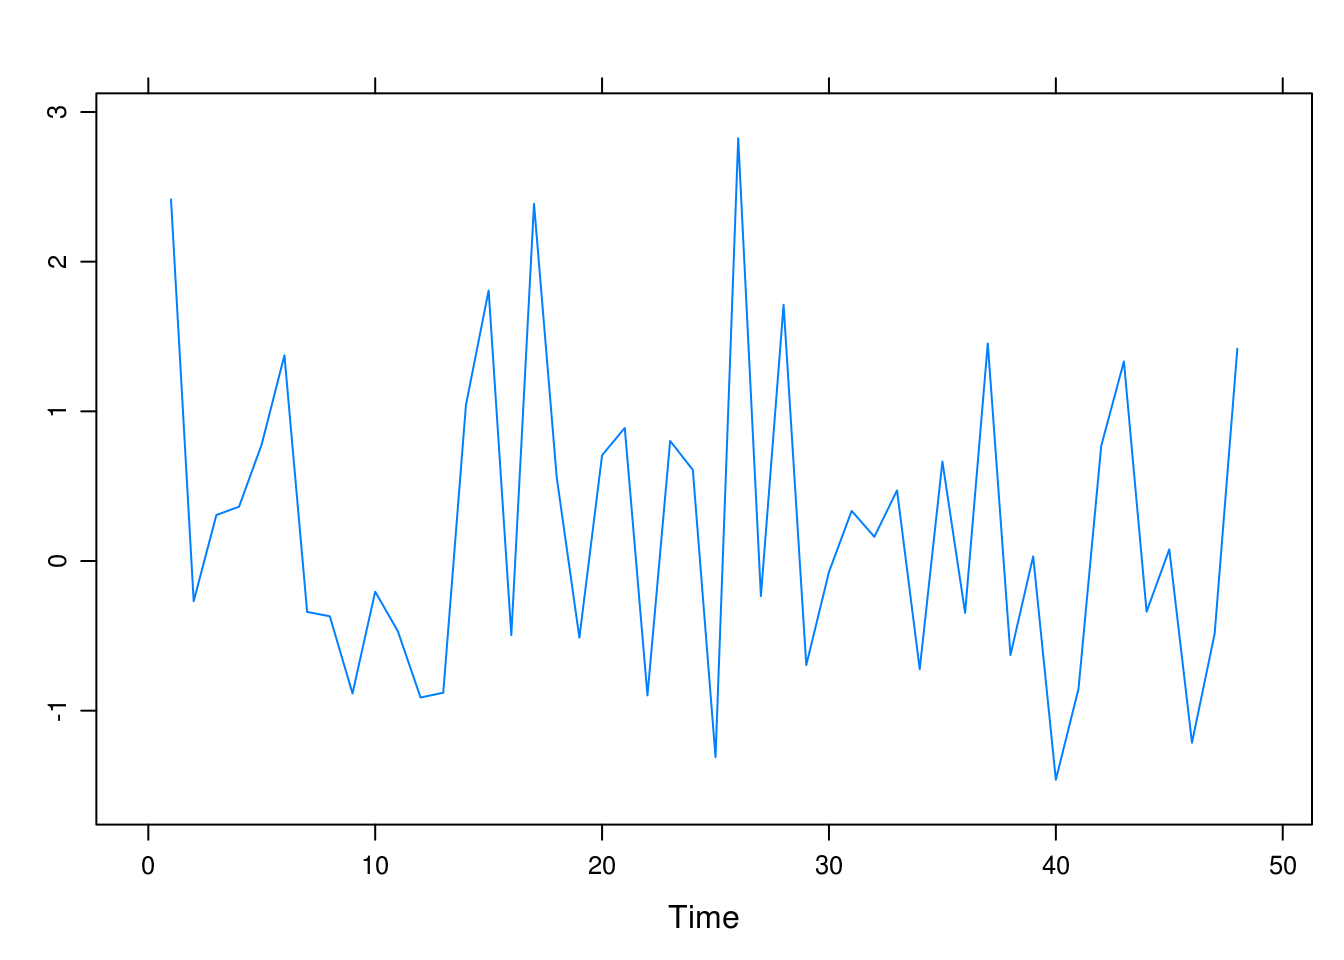
\includegraphics{TSAsolutions_files/figure-latex/unnamed-chunk-3-2.pdf}

As far as we can tell there is no discernable pattern here.

\section{\texorpdfstring{Random, \(\chi^2\)-distributed time
series}{Random, \textbackslash{}chi\^{}2-distributed time series}}\label{random-chi2-distributed-time-series}

\begin{quote}
Simulate a completely random process of length 48 with independent,
chi-square distributed values, each with 2 degrees of freedom. Display
the time series plot. Does it look ``random'' and nonnormal? Repeat this
exercise several times with a new simulation each time.
\end{quote}

\begin{Shaded}
\begin{Highlighting}[]
\KeywordTok{xyplot}\NormalTok{(}\KeywordTok{as.ts}\NormalTok{(}\KeywordTok{rchisq}\NormalTok{(}\DecValTok{48}\NormalTok{, }\DecValTok{2}\NormalTok{)))}
\KeywordTok{xyplot}\NormalTok{(}\KeywordTok{as.ts}\NormalTok{(}\KeywordTok{rchisq}\NormalTok{(}\DecValTok{48}\NormalTok{, }\DecValTok{2}\NormalTok{)))}
\end{Highlighting}
\end{Shaded}

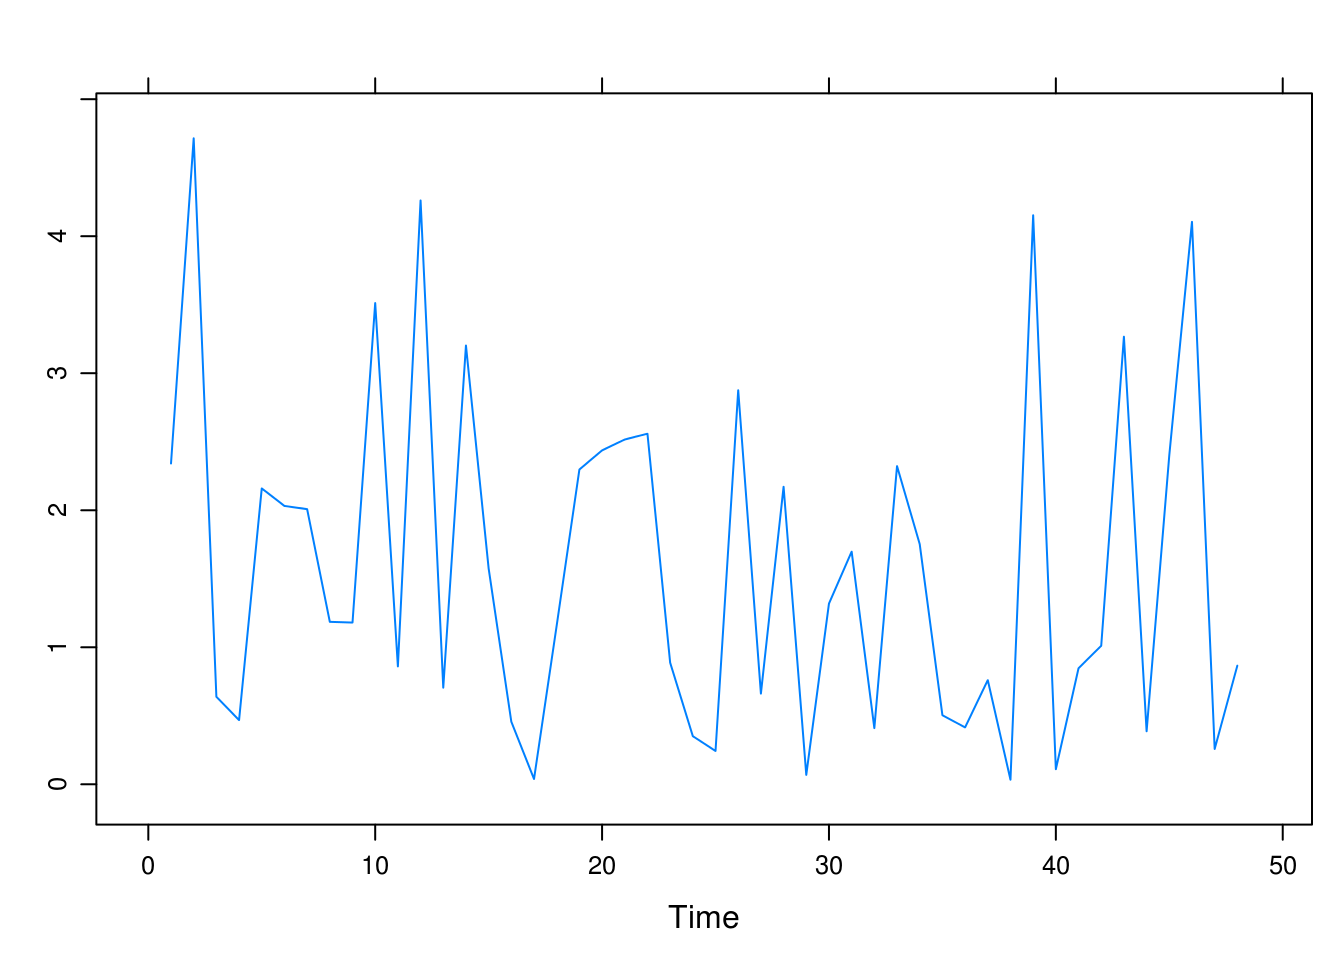
\includegraphics{TSAsolutions_files/figure-latex/unnamed-chunk-4-1.pdf}
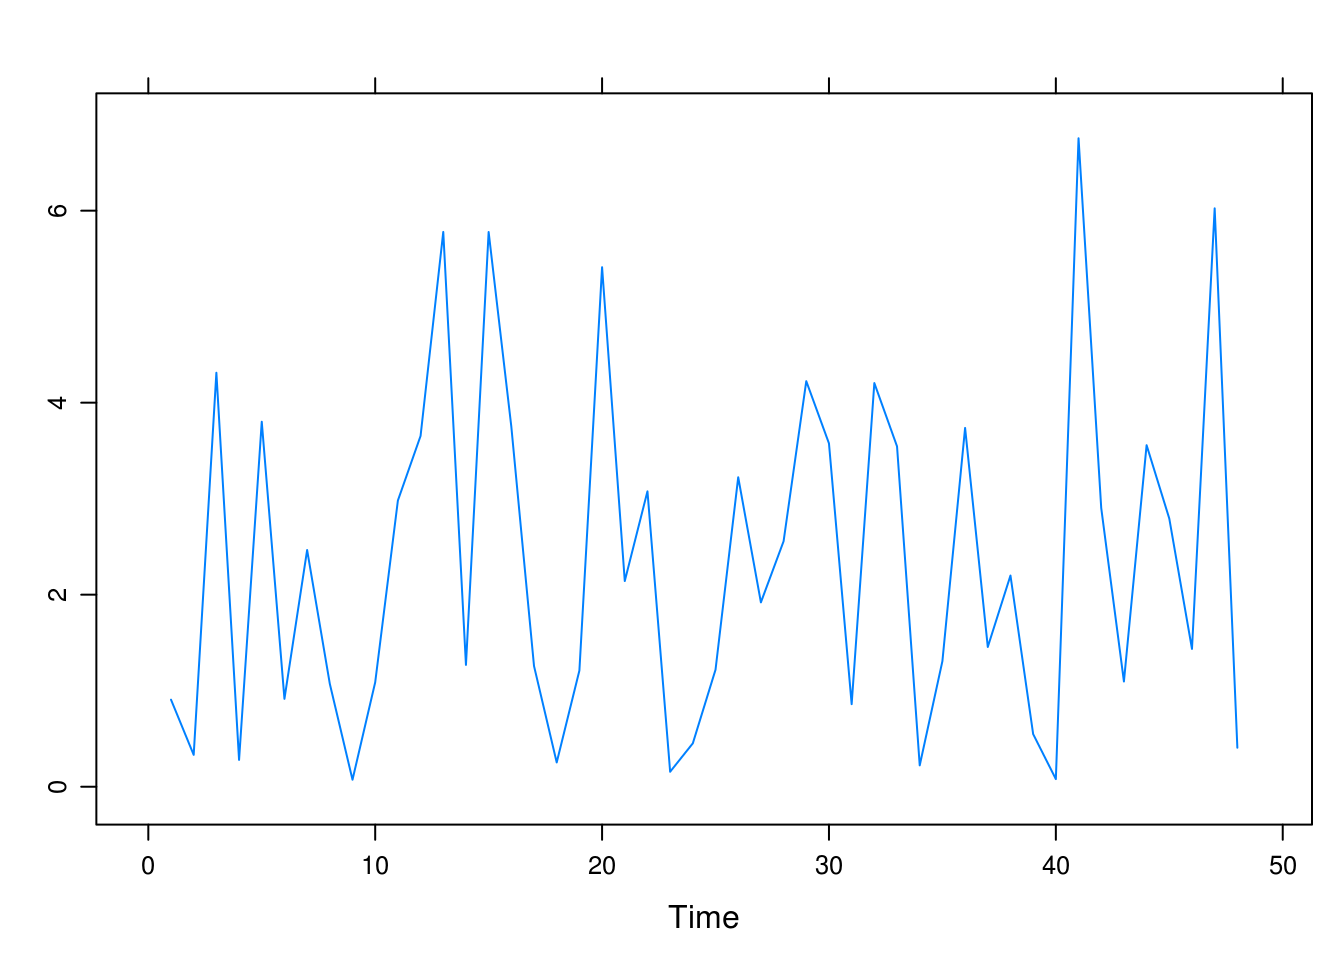
\includegraphics{TSAsolutions_files/figure-latex/unnamed-chunk-4-2.pdf}

The process appears random, though non-normal.

\section{\texorpdfstring{\emph{t}(5)-distributed, random
values}{t(5)-distributed, random values}}\label{t5-distributed-random-values}

\begin{quote}
Simulate a completely random process of length 48 with independent,
t-distributed values each with 5 degrees of freedom. Construct the time
series plot. Does it look ``random'' and nonnormal? Repeat this exercise
several times with a new simulation each time.
\end{quote}

\begin{Shaded}
\begin{Highlighting}[]
\KeywordTok{xyplot}\NormalTok{(}\KeywordTok{as.ts}\NormalTok{(}\KeywordTok{rt}\NormalTok{(}\DecValTok{48}\NormalTok{, }\DecValTok{5}\NormalTok{)))}
\end{Highlighting}
\end{Shaded}

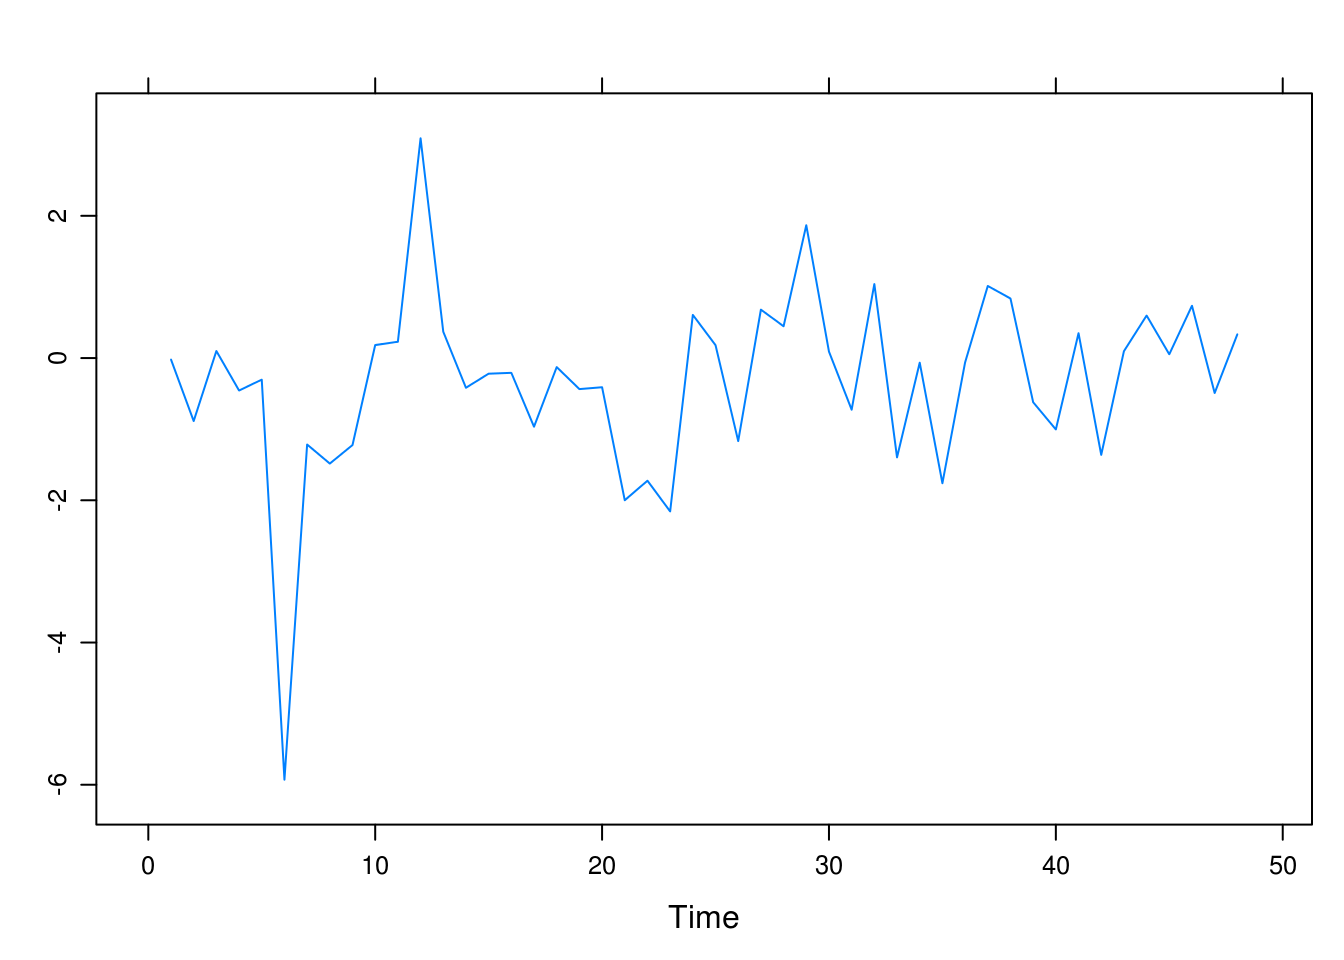
\includegraphics{TSAsolutions_files/figure-latex/unnamed-chunk-5-1.pdf}

\begin{Shaded}
\begin{Highlighting}[]
\KeywordTok{xyplot}\NormalTok{(}\KeywordTok{as.ts}\NormalTok{(}\KeywordTok{rt}\NormalTok{(}\DecValTok{48}\NormalTok{, }\DecValTok{5}\NormalTok{)))}
\end{Highlighting}
\end{Shaded}

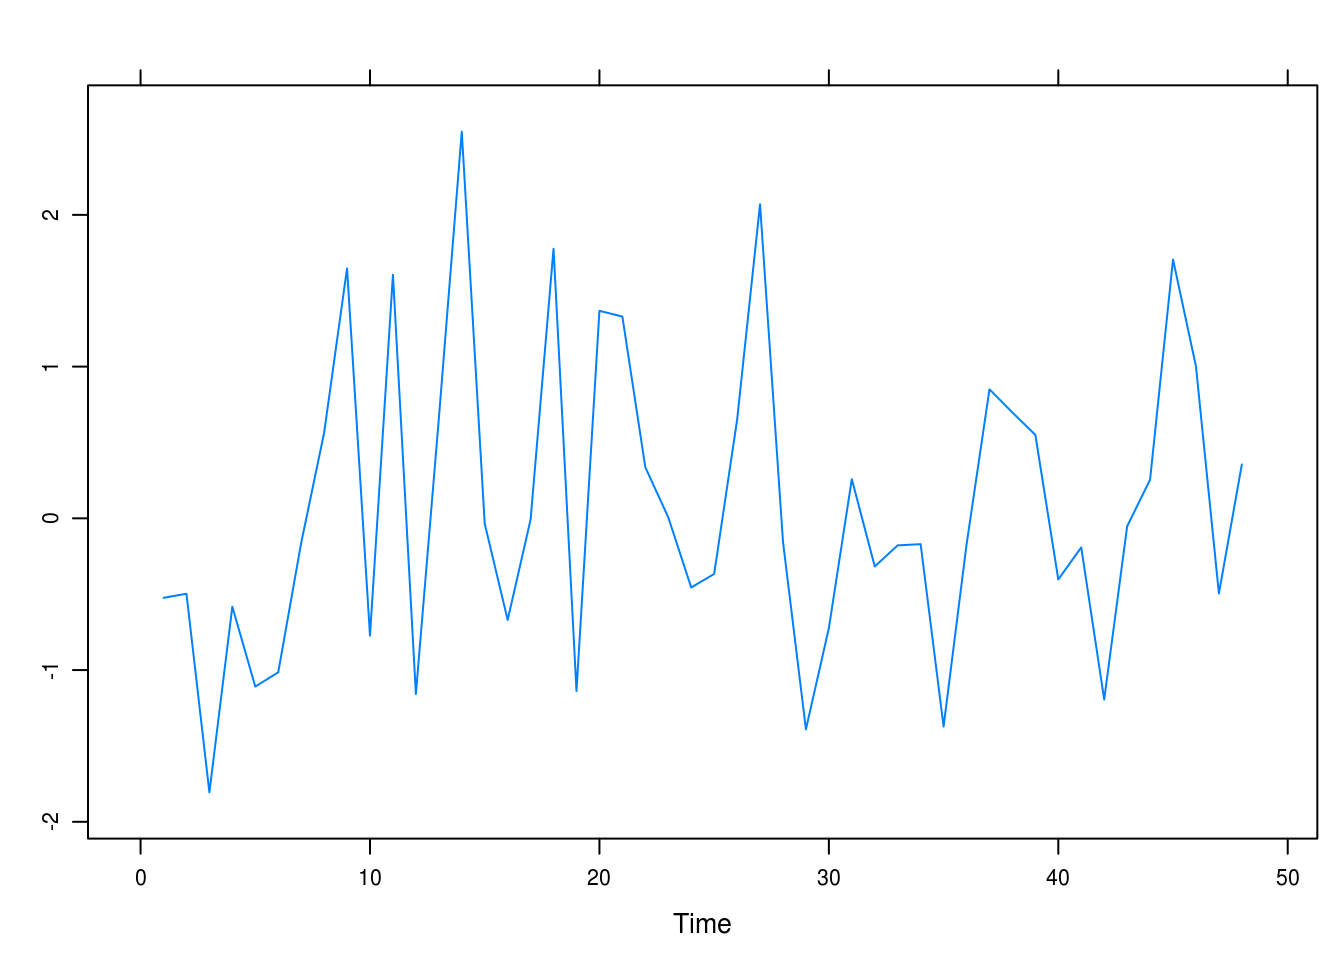
\includegraphics{TSAsolutions_files/figure-latex/unnamed-chunk-5-2.pdf}

It looks random but not normal, though it should be approximately so,
considering the distribution that we have sampled from.

\section{Dubuque temperature series}\label{dubuque-temperature-series}

\begin{quote}
Construct a time series plot with monthly plotting symbols for the
Dubuque temperature series as in Exhibit 1.7, on page 6. The data are in
the file named tempdub.
\end{quote}

\begin{Shaded}
\begin{Highlighting}[]
\KeywordTok{data}\NormalTok{(tempdub)}
\KeywordTok{xyplot}\NormalTok{(tempdub, }\DataTypeTok{ylab =} \StringTok{"Temperature"}\NormalTok{, }\DataTypeTok{xlab =} \StringTok{"Year"}\NormalTok{)}
\end{Highlighting}
\end{Shaded}

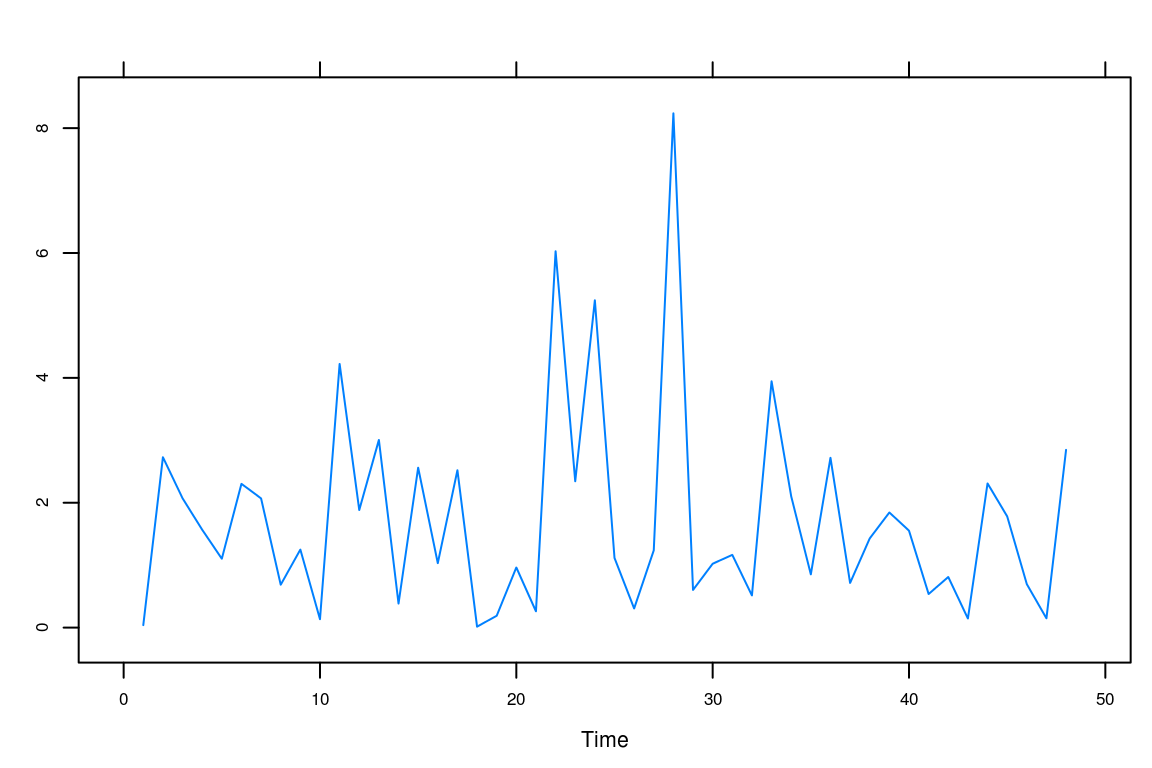
\includegraphics{TSAsolutions_files/figure-latex/unnamed-chunk-6-1.pdf}

\chapter{Fundamental concepts}\label{fundamental-concepts}

\section{Basic properties of expected value and
covariance}\label{basic-properties-of-expected-value-and-covariance}

\subsection*{a}\label{a}
\addcontentsline{toc}{subsection}{a}

\begin{align}
    \text{Cov}[X,Y] & = \text{Corr}[X,Y]\sqrt{Var[X]Var[Y]}\\
                    & = 0.25 \sqrt{9 \times 4} = 1.5 \\
    \text{Var}[X,Y] & = Var[X]+Var[Y]+2Cov[X,Y]\\
                    & = 9 + 4 + 2 \times 3 = 16\\
    \end{align}

\subsection*{b}\label{b}
\addcontentsline{toc}{subsection}{b}

\[\text{Cov}[X, X+Y] = \text{Cov}[X,X] + \text{Cov}[X,Y] =
  \text{Var}[X] + \text{Cov}[X,Y] = 9 + 1.5 = 10.5\]

\subsection*{c}\label{c}
\addcontentsline{toc}{subsection}{c}

\begin{align}
\text{Corr}[X+Y, X-Y] = & \text{Corr}[X,X] + \text{Corr}[X,-Y] +
                          \text{Corr}[Y,X] + \text{Corr}[Y,-Y] \\
                      = & \text{Corr}[Y,X] + \text{Corr}[Y,-Y] \\
                      = & 1 - 0.25 + 0.25 -1 \\
                      = & 0 \\
\end{align}

\section{Dependence and covariance}\label{dependence-and-covariance}

\begin{gather*}
\text{Cov}[X+Y,X-Y] = \text{Cov}[X,X] + \text{Cov}[X,-Y] +
  \text{Cov}[Y,X] + \text{Cov}[Y, -Y] = \\
Var[X] - Cov[X,Y] + Cov[X,Y] - Var[Y] = 0
\end{gather*}

since \(Var[X] = Var[Y]\).

\section{Strict and weak
stationarity}\label{strict-and-weak-stationarity}

\subsection*{a}\label{a-1}
\addcontentsline{toc}{subsection}{a}

We have that

\begin{gather*}
P(Y_{t_1}, Y_{t_2}, \dots, Y_{t_n}) = \\
  P(X_1, X_2, \dots, X_n) = \\
  P(Y_{t_1 - k}, Y_{t_2 - k}, \dots, Y_{t_n - k}),
\end{gather*}

which satisfies our requirement for strict stationarity.

\subsection*{b}\label{b-1}
\addcontentsline{toc}{subsection}{b}

The autocovariance is given by

\begin{gather*}
  \gamma_{t,s}=\text{Cov}[Y_t, Y_s] = \text{Cov}[X,X] = \text{Var}[X] = \sigma^2.
\end{gather*}

\subsection*{c}\label{c-1}
\addcontentsline{toc}{subsection}{c}

\begin{Shaded}
\begin{Highlighting}[]
\KeywordTok{library}\NormalTok{(lattice)}
\NormalTok{tstest <-}\StringTok{ }\KeywordTok{ts}\NormalTok{(}\KeywordTok{runif}\NormalTok{(}\DecValTok{100}\NormalTok{))}

\NormalTok{lattice::}\KeywordTok{xyplot}\NormalTok{(tstest,}
                \DataTypeTok{panel =} \NormalTok{function(x, y, ...) \{}
                  \KeywordTok{panel.abline}\NormalTok{(}\DataTypeTok{h =} \KeywordTok{mean}\NormalTok{(y), }\DataTypeTok{lty =} \DecValTok{2}\NormalTok{)}
                  \KeywordTok{panel.xyplot}\NormalTok{(x, y, ...)}
                \NormalTok{\})}
\end{Highlighting}
\end{Shaded}

\begin{figure}[htbp]
\centering
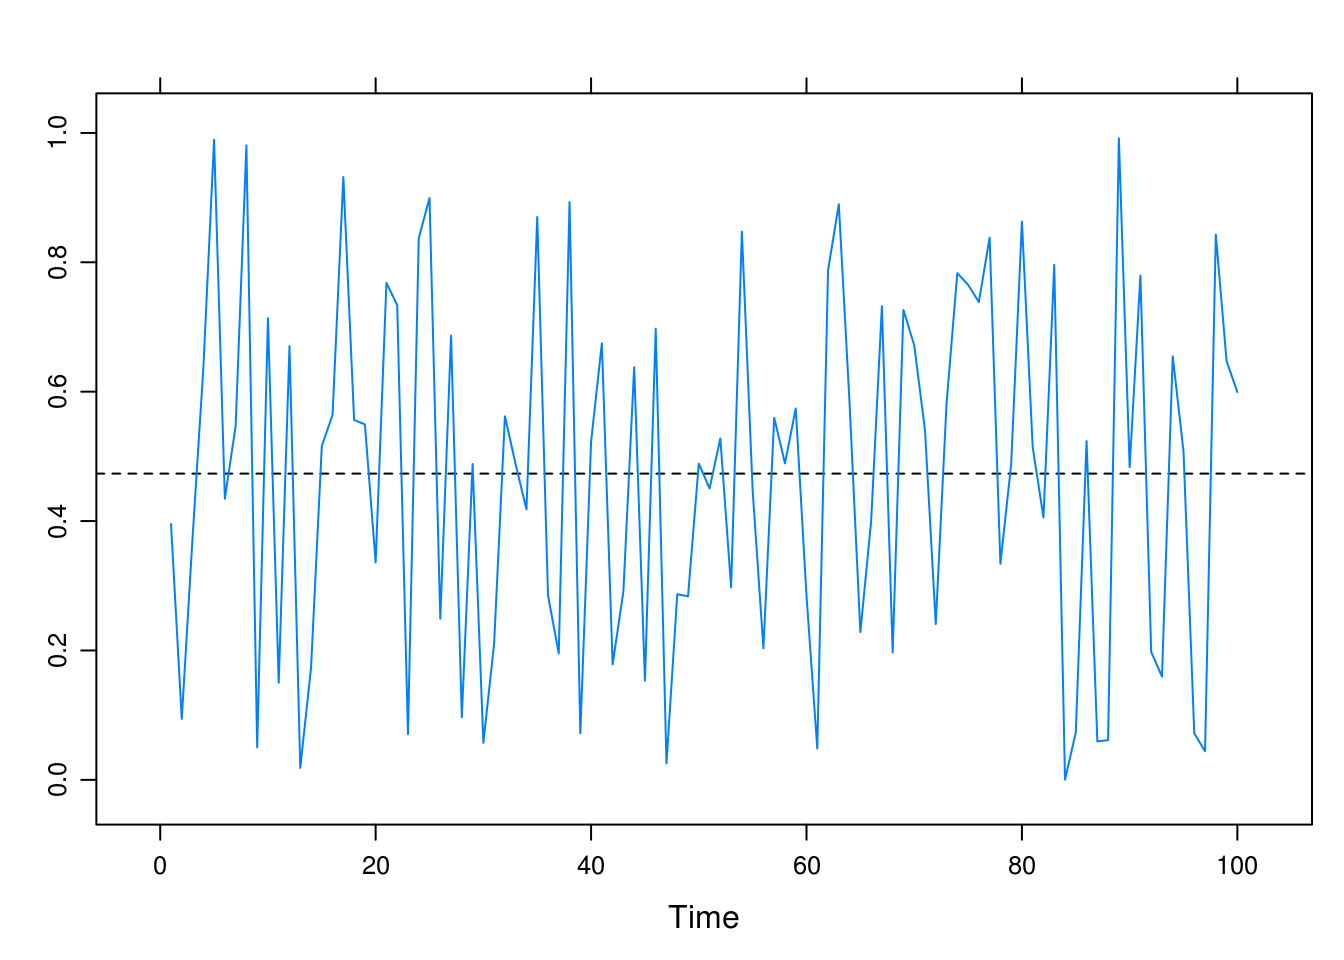
\includegraphics{TSAsolutions_files/figure-latex/unnamed-chunk-7-1.pdf}
\caption{\label{fig:unnamed-chunk-7}A white noise time series: no drift,
independence between observations.}
\end{figure}

\section{Zero-mean white noise}\label{zero-mean-white-noise}

\subsection*{a}\label{a-2}
\addcontentsline{toc}{subsection}{a}

\begin{gather*}
  E[Y_t] = E[e_t+\theta e_{t-1}] = E[e_t] + \theta E[e_{t-1}] = 0 + 0 = 0\\
  V[Y_t] = V[e_t + \theta e_{t-1}] =  V[e_t] + \theta^2 V[e_{t-1}] = \sigma_e^2 + \theta^2 \sigma_e^2 = \sigma_2^2(1 + \theta^2)\\
\end{gather*}

For \(k = 1\) we have

\begin{gather*}
  C[e_t + \theta e_{t-1}, e_{t-1} + \theta e_{t-2}] = \\
  C[e_t,e_{t-1}] + C[e_t, \theta e_{t-2}] + C[\theta e_{t-1}, e_{t-1}] + C[\theta e_{t-1}, \theta e_{t-2}] = \\
  0 + 0 + \theta V[e_{t-1}] + 0 = \theta \sigma_e^2,\\
  \text{Corr}[Y_t, Y_{t-k}] = \frac{\theta \sigma_e^2}{\sqrt{(\sigma_e^2(1+\theta^2))^2}} = \frac{\theta }{1+\theta^2}
\end{gather*}

and for \(k = 0\) we get

\begin{gather*}
  \text{Corr}[Y_t, Y_{t-k}] = \text{Corr}[Y_t, Y_t] = 1
\end{gather*}

and, finally, for \(k > 0\):

\begin{gather*}
  C[e_t + \theta e_{t-1}, e_{t-k} + \theta e_{t-k-1}] = \\
  C[e_t, e_{t-k}] + C[e_t, e_{t-1-k}] + C[\theta e_{t-1}, e_{t-k}] + C[\theta e_{t-1}, \theta e_{t-1-k}] = 0
\end{gather*}

given that all terms are independent. Taken together, we have that

\begin{gather*} \text{Corr}[Y_t, Y_{t-k}] =
  \begin{cases}
    1                            & \quad \text{for } k = 0\\
    \frac{\theta}{1 + \theta^2}  & \quad \text{for } k = 1\\
    0                            & \quad \text{for } k > 1
  \end{cases}.
\end{gather*}

And, as required,

\begin{gather*}
  \text{Corr}[Y_t, Y_{t-k}] =
  \begin{cases}
    \frac{3}{1+3^2} = \frac{3}{10} & \quad \text{if } \theta = 3\\
    \frac{1/3}{1 + (1/3)^2} = \frac{1}{10/3} = \frac{3}{10}  & \quad \text{if } \theta = 1/3
  \end{cases}.
\end{gather*}

\subsection*{b}\label{b-2}
\addcontentsline{toc}{subsection}{b}

No, probably not. Given that \(\rho\) is standardized, we will not be
able to detect any difference in the variance regardless of the values
of k.

\section{Zero-mean stationary series}\label{zero-mean-stationary-series}

\subsection*{a}\label{a-3}
\addcontentsline{toc}{subsection}{a}

\[\mu_t = E[Y_t] = E[5 + 2t + X_t] = 5 + 2E[t] + E[X_t] = 5 + 2t + 0 = 2t + 5\]

\subsection*{b}\label{b-3}
\addcontentsline{toc}{subsection}{b}

\[ \gamma_k = \text{Corr}[5+2t+X_t, 5+2(t-k)+X_{t-k}] =
  \text{Corr}[X_t, X_{t-k}]\]

\subsection*{c}\label{c-2}
\addcontentsline{toc}{subsection}{c}

No, the mean function (\(\mu_t\)) is constant and the aurocovariance
(\(\gamma_{t,t-k}\)) free from \(t\).

\section{Stationary time series}\label{stationary-time-series}

\subsection*{a}\label{a-4}
\addcontentsline{toc}{subsection}{a}

\begin{gather*}\text{Cov}[a + X_t, b + X_{t-k}] =\text{Cov}[X_t, X_{t-k}],\end{gather*}

which is free from \(t\) for all \(k\) because \(X_t\) is stationary.

\subsection*{b}\label{b-4}
\addcontentsline{toc}{subsection}{b}

\begin{gather*}
  \mu_t = E[Y_t] = 
    \begin{cases}
      E[X_t]       & \quad \text{for odd } t\\
      3 + E[X_t]   & \quad \text{for even } t\\
    \end{cases}.
\end{gather*}

Since \(\mu_t\) varies depending on \(t\), \(Y_t\) is not stationary.

\section{First and second-order difference
series}\label{first-and-second-order-difference-series}

\subsection*{a}\label{a-5}
\addcontentsline{toc}{subsection}{a}

\begin{gather*}\mu_t = E[W_t] = E[Y_t - Y_{t-1}] = E[Y_t] - E[Y_{t-1}] = 0\end{gather*}

because \(Y_t\) is stationary.

\begin{gather*}
  \text{Cov}[W_t] = \text{Cov}[Y_t - Y_{t-1}, Y_{t-k} - Y_{t-1-k}] = \\
  \text{Cov}[Y_t, Y_{t-k}] + \text{Cov}[Y_t, Y_{t-1-k}] + \text{Cov}[-Y_{t-k}, Y_{t-k}] + \text{Cov}[-Y_{t-k}, -Y_{t-1-k}]=\\
  \gamma_k-\gamma_{k+1}-\gamma_{k-1}+\gamma_{k} = 2 \gamma_k - \gamma_{k+1} - \gamma_{k-1}. \quad \square
\end{gather*}

\subsection*{b}\label{b-5}
\addcontentsline{toc}{subsection}{b}

In (a), we discovered that the difference between two stationary
processes, \(\triangledown Y_t\) itself was stationary. It follows that
the difference between two of these differences, \(\triangledown^2Y_t\)
is also stationary.

\section{Generalized difference
series}\label{generalized-difference-series}

\begin{align}
  E[W_t] & = c_1E[Y_t]+c_2E[Y_t] + \dots + c_n E[Y_t]\\
         & = E[Y_t](c_1 + c_2 + \dots + c_n),
\end{align}

and thus the expected value is constant. Moreover,

\begin{align}
  \text{Cov}[W_t] & = \text{Cov}[c_1 Y_t + c_2 Y_{t-1} + \dots + c_n Y_{t-k}, c_1 Y_{t-k} + c_2 Y_{t-k-1} + \dots + c_n Y_{t-k-n}] \\
                  & = \sum_{i=0}^n \sum_{j=0}^n c_i c_j \text{Cov}[Y_{t-j}Y_{t-i-k}] \\
                  & = \sum_{i=0}^n \sum_{j=0}^n c_i c_j \gamma_{j-k-i},
\end{align}

which is free of \(t\); consequently, \(W_t\) is stationary.

\section{Zero-mean stationary difference
series}\label{zero-mean-stationary-difference-series}

\subsection*{a}\label{a-6}
\addcontentsline{toc}{subsection}{a}

\begin{gather*}
  E[Y_t] = \beta_0 + \beta_1 t + E[X_t] = \beta_0 + \beta_1 t + \mu_{t_x},
\end{gather*}

which is not free of \(t\) and hence \emph{not} stationary.

\begin{gather*}
  \text{Cov}[Y_t] = \text{Cov}[X_t, X_t-1] = \gamma_{t-1}
\end{gather*}

\begin{gather*}
  E[W_t] = E[Y_t - Y_{t-1}] = E[\beta_0 + \beta_1 t + X_t - (\beta_0 + \beta_1(t-1) + X_{t-1})] =\\
  \beta_0 + \beta_1 t - \beta_0 - \beta_1 t + \beta_1  = \beta_1,
\end{gather*}

is free of \(t\) and, furthermore, we have

\begin{gather*}
  \text{Cov}[W_t] = \text{Cov}[\beta_0 + \beta_1 t + X_t, \beta_0 + \beta_1 (t-1) + X_{t-1}] =\\
  \text{Cov}[X_t, X_{t-1}] = \gamma_k,  
\end{gather*}

which is also free of \(t\), thereby proving that \(W_t\) is stationary.

\subsection*{b}\label{b-6}
\addcontentsline{toc}{subsection}{b}

\begin{gather*}
  E[Y_t] = E[\mu_t + X_t] = \mu_t + \mu_t = 0 + 0 = 0, \quad \text{and}\\
  \text{Cov}[Y_t] = \text{Cov}[\mu_t + X_t, \mu_{t-k} + X_{t-k}] = \text{Cov}[X_t, X_{t-k}] = \gamma_k
\end{gather*}

\begin{gather*}
  \triangledown^m Y_t = \triangledown(\triangledown^{m−1}Y_t)
\end{gather*}

\emph{Currently unsolved.}

\section{Zero-mean, unit-variance
process}\label{zero-mean-unit-variance-process}

\subsection*{a}\label{a-7}
\addcontentsline{toc}{subsection}{a}

\begin{gather*}
  \mu_t = E[Y_t] = E[\mu_t + \sigma_t X_t] = \mu_t + \sigma_t E[X_t] = \mu_t + \sigma_t \times 0 = \mu_t\\
  \gamma_{t,t-k} = \text{Cov}[Y_t] = \text{Cov}[\mu_t + \sigma_t X_t, \mu_{t-k} + \sigma_{t-k} X_{t-k}] = 
    \sigma_t \sigma_{t-k} \text{Cov}[X_t, X_{t-k}] = \sigma_t \sigma_{t-k} \rho_k
\end{gather*}

\subsection*{b}\label{b-7}
\addcontentsline{toc}{subsection}{b}

First, we have

\begin{gather*}
  \text{Var}[Y_t] = \text{Var}[\mu_t + \sigma_t X_t] = 0 + \sigma_t^2 \text{Var}[X_t] = \sigma_t^2 \times 1 = \sigma_t^2
\end{gather*}

since \(\{X_t\}\) has unit-variance. Futhermore,

\begin{gather*}
  \text{Corr}[Y_t, Y_{t-k}] = \frac{\sigma_t \sigma_{t-k} \rho_k}{\sqrt{\text{Var}[Y_t]\text{Var}[Y_{t-k}]}} = 
    \frac{\sigma_t \sigma_{t-k}\rho_k}{\sigma_t \sigma_{t-k}} = \rho_k,
\end{gather*}

which depends only on the time lag, \(k\). However, \(\{Y_t\}\) is not
necessarily stationary since \(\mu_t\) may depend on \(t\).

\subsection*{c}\label{c-3}
\addcontentsline{toc}{subsection}{c}

Yes, \(\rho_k\) might be free from \(t\) but if \(\sigma_t\) is not, we
will have a non-stationary time series with autocorrelation free from
\(t\) and constant mean.

\section{Drift}\label{drift}

\subsection*{a}\label{a-8}
\addcontentsline{toc}{subsection}{a}

\begin{gather*}
  \text{Cov}[X_t, X_{t-k}] = \gamma_k\\
  E[X_t] = 3t
\end{gather*}

\(\{X_t\}\) is not stationary because \(\mu_t\) varies with \(t\).

\subsection*{b}\label{b-8}
\addcontentsline{toc}{subsection}{b}

\begin{gather*}
  E[Y_t] = 3 - 3t+E[X_t] = 7 - 3t - 3t = 7\\
  \text{Cov}[Y_t, Y_{t-k}] = \text{Cov}[7-3t+X_t,7-3(t-k)+X_{t-k}] = \text{Cov}[X_t, X_{t-k}] = \gamma_k
\end{gather*}

Since the mean function of \(\{Y_t\}\) is constant (7) and its
autocovariance free of \(t\), \(\{Y_t\}\) is stionary.

\section{Periods}\label{periods}

\begin{gather*}
  E[Y_t] = E[e_t - e_{t-12}] = E[e_t] - E[e_{t-12}] = 0\\
  \text{Cov}[Y_t, Y_{t-k}] = \text{Cov}[e_t - e_{t-12}, e_{t-k} - e_{t-12-k}] =\\
  \text{Cov}[e_t, e_{t-k}] - \text{Cov}[e_t, e_{t-12-k}] - \text{Cov}[e_{t-12}, e_{t-k}] + \text{Cov}[e_{t-12}, e_{t-12-k}]
\end{gather*}

Then, as required, we have

\begin{gather*} \text{Cov}[Y_t, Y_{t-k}] =
  \begin{cases}
    \text{Cov}[e_t, e_{t-12}] - \text{Cov}[e_t, e_t] -\\ \text{Cov}[e_{t-12}, e_{t-12}] + \text{Cov}[e_{t-12},e_t] =\\
      \text{Var}[e_t] - \text{Var}[e_{t-12}] \neq 0 & \quad \text{for }  k=12\\
      \\
    \text{Cov}[e_t, e_{t-k}] - \text{Cov}[e_t, e_{t-12-k}] -\\ \text{Cov}[e_{t-12}, e_{t-k}] + \text{Cov}[e_{t-12}, e_{t-12-k}] =\\
    0 + 0 + 0 + 0 = 0 & \quad \text{for } k \neq 12
  \end{cases}
\end{gather*}

\section{Drift, part 2}\label{drift-part-2}

\subsection*{a}\label{a-9}
\addcontentsline{toc}{subsection}{a}

\begin{gather*}
  E[Y_t] = E[e_t - \theta e_{t-1}^2] = E[e_t] - \theta E[e_{t-1}^2] = 0 - \theta \text{Var}[e_{t-1}] = -\theta \sigma_e^2
\end{gather*}

And thus the requirement of constant variance is fulfilled. Moreover,

\begin{gather*}
  \text{Var}[Y_t] = \text{Var}[e_t-\theta e_{t-1}^2] = \text{Var}[e_t] + \theta^2 \text{Var}[e_{t-1}^2] = \sigma_e^2 + \theta^2 (E[e_{t-1}^4] - E[e_{t-1}^2]^2),
\end{gather*}

where

\begin{gather*}
  E[e_{t-1}^4] = 3\sigma_e^4 \quad \text{and} \quad E[e_{t-1}^2 ]^2 = \sigma_e^4,
\end{gather*}

gives us

\begin{gather*}
  \text{Var}[Y_t] = \sigma_e^2 + \theta(3\sigma_e^4 - \sigma_e^2) = \sigma_e^2 + 2 \theta^2 \sigma_e^4
\end{gather*}

and

\begin{gather*}
  \text{Cov}[Y_t, Y_{t-1}] = \text{Cov}[e_t - \theta e_{t-1}^2, e_{t-1} - \theta e_{t-2}^2] = \\
  \text{Cov}[e_t, e_{t-1}] + \text{Cov}[e_t, - \theta e_{t-2}^2] + \text{Cov}[- \theta e_{t-1}^2, e_{t-1}]
    \text{Cov}[-\theta e_{t-1}^2, - \theta e_{t-2}^2] =\\
  \text{Cov}[e_t, e_{t-1}] - \theta \text{Cov}[e_t, e_{t-2}^2] - \theta \text{Cov}[e_{t-1}^2, e_{t-1}] +
    \theta^2 \text{Cov}[e_{t-1}^2, e_{t-2}^2] = \\
  -\theta \text{Cov}[e_{t-1}^2, e_{t-1}] = -\theta (E[e_{t-1}^3] + \mu_{t-1} + \mu_t) = 0
\end{gather*}

which means that the autocorrelation function \(\gamma_{t,s}\) also has
to be zero.

\subsection*{b}\label{b-9}
\addcontentsline{toc}{subsection}{b}

The autocorrelation of \(\{Y_t\}\) is zeor and its mean function is
constant, thus \(\{Y_t\}\) must be stationary.

\section{Stationarity, again}\label{stationarity-again}

\subsection*{a}\label{a-10}
\addcontentsline{toc}{subsection}{a}

\begin{gather*}
  E[Y_t]= E[\theta_0 +  t e_t] = \theta_0 + E[e_t] = \theta_0+t \times 0 = \theta_0\\
\text{Var}[Y_t] = \text{Var}[\theta_0] + \text{Var}[t e_t] = 0 + t^2\sigma_e^2 = t^2\sigma_e^2
\end{gather*}

So \(\{Y_t\}\) is not stationary.

\subsection*{b}\label{b-10}
\addcontentsline{toc}{subsection}{b}

\begin{gather*}
  E[W_t] = E[\triangledown Y_t] = E[\theta_0 + te_t - \theta_0 - (t-1)e_{t-1}] =
    tE[e_t] - tE[e_{t-1} + E[e_{t-1}] = 0 \\
  \text{Var}[\triangledown Y_t] = \text{Var}[t e_t] = - \text{Var}[(t-1)e_{t-1}] = 
    t^2 \sigma_e^2 - (t-1)^2 \sigma_e^2 = \sigma_e^2 (t^2 - t^2 + 2t - 1) = (2t-1)\sigma_e^2,
\end{gather*}

which varies with \(t\) and means that \(\{W_t\}\) is not stationary.

\subsection*{c}\label{c-4}
\addcontentsline{toc}{subsection}{c}

\begin{gather*}
  E[Y_t] = E[e_t e_{t-1}] = E[e_t] E[e_{t-1}] = 0\\
  \text{Cov}[Y_t, Y_{t-1}] = \text{Cov}[e_t e_{t-1}, e_{t-1} e_{t-2}] = E[(e_t e_{t-1} - \mu_t^2)(e_{t-1} e_{t-2} - \mu_t^2)] =\\
  E[e_t]E[e_{t-1}]E[e_{t-1}]E[e_{t-2}] = 0
\end{gather*}

Both the covariance and the mean function are zero, hence the process is
stationary.

\section{Random variable, zero mean}\label{random-variable-zero-mean}

\subsection*{a}\label{a-11}
\addcontentsline{toc}{subsection}{a}

\(E[Y_t] = (-1)^tE[X] = 0\)

\subsection*{b}\label{b-11}
\addcontentsline{toc}{subsection}{b}

\(\text{Cov}[Y_t, Y_{t-k}] = \text{Cov}[(-1)^tX, (-1)^{t-k}X] = (-1)^{2t-k}\text{Cov}[X, X] = (-1)^k \text{Var}[X] = (-1)^k\sigma_t^2\)

\subsection*{c}\label{c-5}
\addcontentsline{toc}{subsection}{c}

Yes, the covariance is free of \(t\) and the mean is constant.

\section{Mean and variance}\label{mean-and-variance}

\begin{gather*}
  E[Y_t] = E[A + X_t] = E[A] + E[X_t] = \mu_A + \mu_X\\
  \text{Cov}[Y_t, Y_{t-k}] = \text{Cov}[A + X_t, A+ X_{t-k}] = \\
  \text{Cov}[A, A] + \text{Cov}[A, X_{t-k}] + \text{Cov}[X_t, A] + \text{Cov}[X_t, X_{t-k}] = \sigma_A^2 + \gamma_{k_k}
\end{gather*}

\section{Variance of sample mean}\label{variance-of-sample-mean}

\begin{gather*}
  \text{Var}[\bar{Y}] = \text{Var}\left[ \frac{1}{n} \sum_{t=1}^n Y_t \right] = \frac{1}{n^2} \text{Var}\left[ \sum_{t=1}^n Y_t \right] = \\
  \frac{1}{n^2}\text{Cov}\left[ \sum_{t=1}^n Y_t, \sum_{s=1}^n Y_s \right] = \frac{1}{n^2} \sum_{t=1}^n \sum_{s=1}^n \gamma_{t-s}
\end{gather*}

Setting \(k = t-s, j = t\) gives us

\begin{gather*}
  \text{Var}[\bar{Y}] = \frac{1}{n^2} \sum_{j=1}^n \sum_{j-k=1}^n \gamma_k = \frac{1}{n^2} \sum_{j=1}^n \sum_{j=k+1}^{n+k} \gamma_k = \\
  \frac{1}{n^2} \left( \sum_{k=1}^{n-1} \sum_{j=k+1}^{n} \gamma_k + \sum_{k=-n+1}^0 \sum_{j=1}^{n+k} \gamma_k \right) = \\
  \frac{1}{n^2} \left( \sum_{k=1}^{n-1} (n-k)\gamma_k + \sum_{k=-n+1}^0 (n+k)\gamma_k \right) = \\
  \frac{1}{n^2} \sum_{k=-n+1}^{n-1} \left( (n-k)\gamma_k + (n+k)\gamma_k \right) = \\
  \frac{1}{n^2} \sum_{k=-n+1}^{n-1} (n-|k|)\gamma_k = \frac{1}{n} \sum_{k=-n+1}^{n-1} \left(1-\frac{|k|}{n}\right)\gamma_k \quad \square
\end{gather*}

\section{Sample variance}\label{sample-variance}

\subsection*{a}\label{a-12}
\addcontentsline{toc}{subsection}{a}

\begin{gather*}
  \sum_{t=1}^n (Y_t - \mu)^2 = \sum_{t=1}^n((Y_t - \bar{Y}) + (\bar{Y} - \mu))^2 = \\
  \sum_{t=1}^n ((Y_t - \bar{Y})^2 - 2(Y_t - \bar{Y})(\bar{Y}- \mu) + (\bar{Y} - \mu)^2) = \\
  n(\bar{Y} - \mu)^2 + 2(\bar{Y} - \mu)\sum_{t=1}^n (Y_t - \bar{Y}) + \sum_{t=1}^n (Y_t - \bar{Y})^2  = \\
  n(\bar{Y} - \mu)^2 + \sum_{t=1}^n(Y_t - \bar{Y})^2 \quad \square
\end{gather*}

\subsection*{b}\label{b-12}
\addcontentsline{toc}{subsection}{b}

\begin{gather*}
  E[s^2] = E\left[\frac{n}{n-1} \sum_{t=1}^n (Y_t - \bar{Y})^2 \right] =
    \frac{n}{n-1} E\left[\sum_{t=1}^n \left( (Y_t-\mu)^2  + n(\bar{Y} - \mu)^2 \right)\right] = \\
  \frac{n}{n-1} \sum_{t=1}^n \left( E[(Y_t-\mu)^2]  + nE[(\bar{Y} - \mu)^2] \right) = 
    \frac{1}{n-1} \left( n\text{Var}[Y_t] - n\text{Var}[\bar{Y}] \right) = \\
  \frac{n}{n-1} \gamma_0 - \frac{n}{n-1} \text{Var}[\bar{Y}] =
    \frac{1}{n-1} \left( n \gamma_0 - n \left( \frac{\gamma_0}{n} + \frac{2}{n} \sum_{k=1}^{n-1} \left( 1 - \frac{k}{n} \right) \gamma_k\right) \right) = \\
  \frac{1}{n-1} \left( n \gamma_0 - \gamma_0 + 2 \sum_{k=1}^{n-1} \left( 1 - \frac{k}{n} \right) \gamma_k\right) = 
    \frac{1}{n-1} \left( \gamma_0(n-1) + 2 \sum_{k=1}^{n-1} \left( 1 - \frac{k}{n} \right) \gamma_k\right) = \\
  \gamma_0 + \frac{2}{n-1} \sum_{k=1}^{n-1} \left( 1 - \frac{k}{n} \right) \gamma_k \quad \square
\end{gather*}

\subsection*{c}\label{c-6}
\addcontentsline{toc}{subsection}{c}

Since \(\gamma_k = 0\) for \(k \neq 0\), in our case for all \(k\), we
have

\begin{gather*}
  E[s^2] = \gamma_0 - \frac{2}{n-1} \sum_{t=1}^n \left( 1 - \frac{k}{n} \right) \times 0 = \gamma_0
\end{gather*}

\section{Random walk with drift}\label{random-walk-with-drift}

\subsection*{a}\label{a-13}
\addcontentsline{toc}{subsection}{a}

\begin{gather*}
  Y_{1} = \theta_0 + e_1\\
  Y_{2} = \theta_0 + \theta_0 + e_2 + e_1\\
  Y_{t} = \theta_0 + \theta_0 + \dots + \theta_0 + e_{t} + e_{t-1} + \dots+ e_1 = \\
  Y_{t} = t \theta_0 + e_t + e_{t-1} + \dots + e_1 \quad \square
\end{gather*}

\subsection*{b}\label{b-13}
\addcontentsline{toc}{subsection}{b}

\begin{gather*}
  \mu_t = E[Y_t] = E[t \theta_0 + e_t + e_{t-1} + \dots + e_1] = t\theta_0 + E[e_t] + E[e_{t-1}] + \dots + E[e_1] = \\
  t\theta_0 + 0 + 0 + \dots + 0 = t \theta_0
\end{gather*}

\subsection*{c}\label{c-7}
\addcontentsline{toc}{subsection}{c}

\begin{gather*}
  \gamma_{t,t-k} = \text{Cov}[Y_t, Y_{t-k}] = \text{Cov}[t\theta_0 + e_t, + e_{t-1} + \dots + e_1, (t-k)\theta_0 + e_{t-k}, + e_{t-1-k} + \dots + e_1] = \\
   \text{Cov}[e_{t-k}, + e_{t-1-k} + \dots + e_1, e_{t-k}, + e_{t-1-k} + \dots + e_1] \quad \text{(since all other terms are 0)} =\\
   \text{Var}[e_{t-k}, + e_{t-1-k} + \dots + e_1, e_{t-k}, + e_{t-1-k} + \dots + e_1] = (t-k)\sigma_e^2
\end{gather*}

\section{Random walk}\label{random-walk}

\subsection*{a}\label{a-14}
\addcontentsline{toc}{subsection}{a}

\begin{gather*}
  \mu_1 = E[Y_1] = E[e_1] = 0\\
  \mu_2 = E[Y_2] = E[Y_1 - e_2] = E[Y_1] - E[e_2] = 0 - 0 = 0\\
  \dots\\
  \mu_{t-1} = E[Y_{t-1}] = E[Y_{t-2} - e_{t-1}] = E[Y_{t-2}] - E[e_{t-1}] = 0 \\
  \mu_t = E[Y_t] = E[Y_{t-1} - e_t] = E[Y_t] - E[e_t] = 0,
\end{gather*}

which implies \(\mu_t = \mu_{t-1}\quad\) Q.E.D.

\subsection*{b}\label{b-14}
\addcontentsline{toc}{subsection}{b}

\begin{gather*}
  \text{Var}[Y_1] = \sigma_e^2\\
  \text{Var}[Y_2] = \text{Var}[Y_1 - e_2] = \text{Var}[Y_1] + \text{Var}[e_1] = \sigma_e^2 +  \sigma_e^2 = 2\sigma_e^2\\
  \dots\\
  \text{Var}[Y_{t-1}] = \text{Var}[Y_{t-2} - e_{t-1}] = \text{Var}[Y_{t-2}] + \text{Var}[e_{t-1}]  = (t-1)\sigma_e^2\\
  \text{Var}[Y_t] = \text{Var}[Y_{t-1} - e_t] = \text{Var}[Y_{t-1}] + \text{Var}[e_t]  = (t-1)\sigma_e^2 + \sigma_e^2 = t\sigma_e^2 \quad \square
\end{gather*}

\subsection*{c}\label{c-8}
\addcontentsline{toc}{subsection}{c}

\begin{gather*}
  \text{Cov}[Y_t, Y_s] = \text{Cov}[Y_t, Y_t+e_{t+1}+e_{t+2}+ \dots + e_s] = \text{Cov}[Y_t, Y_t] = \text{Var}[Y_t] = t\sigma_e^2
\end{gather*}

\section{Random walk with random starting
value}\label{random-walk-with-random-starting-value}

\subsection*{a}\label{a-15}
\addcontentsline{toc}{subsection}{a}

\begin{gather*}
  E[Y_t] = E[Y_0+e_t+e_{t-1}+\dots+e_1] = \\
  E[Y_0] + E[e_t] + E[e_{t-1}] + E[e_{t-2}] + \dots + E[e_1] = \\
  \mu_0 + 0 + \dots + 0 = \mu_0 \quad \square
\end{gather*}

\subsection*{b}\label{b-15}
\addcontentsline{toc}{subsection}{b}

\begin{gather*}
  \text{Var}[Y_t] = \text{Var}[Y_0 + e_t + e_{t-1} + \dots + e_1] = \\
  \text{Var}[Y_0] + \text{Var}[e_t] + \text{Var}[e_{t-1}] + \dots + \text{Var}[e_1] = \\
  \sigma_0^2+t\sigma_e^2 \quad \square
\end{gather*}

\subsection*{c}\label{c-9}
\addcontentsline{toc}{subsection}{c}

\begin{gather*}
  \text{Cov}[Y_t, Y_s] = \text{Cov}[Y_t, Y_t+e_{t+1}+e_{t+2}+ \dots + e_s] = \\
  \text{Cov}[Y_t, Y_t] = \text{Var}[Y_t] = \sigma_0^2+t\sigma_e^2 \quad \square
\end{gather*}

\subsection*{d}\label{d}
\addcontentsline{toc}{subsection}{d}

\begin{gather*}
  \text{Corr}[Y_t, Y_s] = \frac{\sigma_0^2+t\sigma_e^2}{\sqrt{(\sigma_0^2+t\sigma_e^2)(\sigma_0^2+s\sigma_e^2)}} = 
    \sqrt{\frac{\sigma_0^2+t\sigma_e^2}{\sigma_0^2+s\sigma_e^2}} \quad \square
\end{gather*}

\section{Asymptotic stationarity}\label{asymptotic-stationarity}

\subsection*{a}\label{a-16}
\addcontentsline{toc}{subsection}{a}

\begin{gather*}
  E[Y_1] = E[e_1] = 0\\
  E[Y_2] = E[cY_{1}+e_2] = cE[Y_1] + E[e_2] = 0\\
  \dots\\
  E[Y_t] = E[cY_{t-1}+e_t] = cE[Y_{t-1}] + E[e_t] = 0\quad \square
\end{gather*}

\subsection*{b}\label{b-16}
\addcontentsline{toc}{subsection}{b}

\begin{gather*}
  \text{Var}[Y_1] = \text{Var}[e_1] = \sigma_e^2\\
  \text{Var}[Y_2] = \text{Var}[cY_{1} + e_2] = c^2\text{Var}[Y_{t-1}] + \text{Var}[e_2] = c^2\sigma_e^2 + \sigma_e^2 = \sigma_e^2(1 + c^2)\\
  \dots\\
  \text{Var}[Y_t] = \sigma_e^2(1 + c^2 + c^4 + \dots + c^{2t-2}) \quad\square
\end{gather*}

\(\{Y_t\}\) is not stationary, given that its variance varies with
\(t\).

\subsection*{c}\label{c-10}
\addcontentsline{toc}{subsection}{c}

\begin{gather*}
  \text{Cov}[Y_t, Y_{t-1}] = \text{Cov}[cY_{t-1} + e_t, Y_{t-1}] = c\text{Cov}[Y_{t-1}, Y_{t-1}] = c\text{Var}[Y_{t-1}]\quad \text{giving}\\
  \text{Corr}[Y_t, Y_{t-1}] = \frac{c\text{Var}[Y_{t-1}]}{\sqrt{\text{Var}[Y_t]\text{Var}[Y_{t-1}]}} =
    c \sqrt{\frac{\text{Var}[Y_{t-1}]}{\text{Var}[Y_t]}}\quad\square
\end{gather*}

And, in the general case,

\begin{gather*}
  \text{Cov}[Y_t, Y_{t-k}] = \text{Cov}[cY_{t-1}+e_t, Y_{t-k}] = \\
  c\text{Cov}[cY_{t-2} + e_{t-1}, Y_{t-k}] =\\
  c^3\text{Cov}[Y_{t-2} + e_{t-1}, Y_{t-k}] = \dots\\ = c^k\text{Var}[Y_{t-k}]
\end{gather*}

giving

\begin{gather*}
  \text{Corr}[Y_t, Y_{t-k}] = \frac{c^k\text{Var}[Y_{t-k}]}{\sqrt{\text{Var}[Y_t]\text{Var}[Y_{t-k}]}} =
    c^k \sqrt{\frac{\text{Var}[Y_{t-k}]}{\text{Var}[Y_t]}}\quad\square
\end{gather*}

\subsection*{d}\label{d-1}
\addcontentsline{toc}{subsection}{d}

\begin{gather*}
  \text{Var}[Y_t] = \sigma_e^2(1+c^2+c^4+\dots+c^{2t-2}) = \sigma_e^2\sum_{t=1}^{n}c^{2(t-1)}=\sigma_e^2 \sum_{t=0}^{n-1} c^{2t} =
    \sigma_e^2 \frac{1-c^{2t}}{1-c^2}
\end{gather*}

And because

\begin{gather*}
\lim_{t \rightarrow \infty} \sigma_e^2 \frac{1-c^{2t}}{1-c^2} = \sigma_e^2 \frac{1}{1-c^2}\quad\text{since }|c| < 1,
\end{gather*}

which is free of \(t\), \(\{Y_t\}\) can be considered
\emph{asymptotically} stationary.

\subsection*{e}\label{e}
\addcontentsline{toc}{subsection}{e}

\begin{gather*}
  Y_t = c(cY_{t-2} + e_{t-1}) + e_t = \dots = e_t+ce_{t-1} + c^2e_{t-2} + \dots + c^{t-2}e_2+ \frac{c^{t-1}}{\sqrt{1-c^2}}e_1\\
  \text{Var}[Y_t] = \text{Var}[e_t+ce_{t-1}+c^2e_{t-2}+\dots+c^{t-2}e_2+\frac{c^{t-1}}{\sqrt{1-c^2}}e_1] =\\
  \text{Var}[e_t] + c^2\text{Var}[e_{t-1}]+c^4 \text{Var}[e_{t-2}] + \dots + c^{2(t-2)}\text{Var}[e_2]+\frac{c^{2(t-1)}}{1-c^2}\text{Var}[e_1] =\\
  \sigma_e^2(1 + c^2 + c^4 + \dots + c^{2(t-2)} + \frac{c^{2(t-1)}}{1-c^2}) =\sigma_e^2\left( \sum_{t=1}^{n}c^{2(t-1)} - c^{2(t-1)} + \frac{c^{2(t-1)}}{1-c^2}\right)= \\
  \sigma_e^2 \frac{1-c^{2t}+c^{2t-2+2}}{1-c^2} = \sigma_e^2 \frac{1}{1-c^2} \quad \square
\end{gather*}

Futhermore,

\begin{gather*}
  E[Y_1] = E\left[\frac{e_1}{\sqrt{1-c^2}}\right] = \frac{E[e_1]}{\sqrt{1-c^2}} = 0\\
  E[Y_2] = E[cY_{1} + e_2] = cE[Y_{1}] = 0\\
  \dots \\
  E[Y_t] = E[cY_{t-1} + e_2] = cE[Y_{t-1}] = 0,\\
\end{gather*}

which satisfies our first requirement for weak stationarity. Also,

\begin{gather*}
  \text{Cov}[Y_t,Y_{t-k}] = \text{Cov}[cY_{t-1} + e_t, Y_{t-1}] = c^k\text{Var}[Y_{t-1}] =\\
    c^k \frac{\sigma_e^2}{1-c^2},
\end{gather*}

which is free of \(t\) and hence \(\{Y_t\}\) is now stationary.

\section{Stationarity in sums of stochastic
processes}\label{stationarity-in-sums-of-stochastic-processes}

\begin{gather*}
  E[W_t] = E[Z_t + Y_t] = E[Z_t] + Y[Z_t] = \mu_{Z_t} + \mu_{Y_s}
\end{gather*}

Since both processes are stationary -- and hence their sums are constant
-- the sum of both processes must also be constant.

\begin{gather*}
  \text{Cov}[W_t, W_{t-k}] = \text{Cov}[Z_t + Y_t, Z_{t-k} + Y_{t-k}] = \\
  \text{Cov}[Z_t, Z_{t-k}] + \text{Cov}[Z_t, Y_{t-k}] + \text{Cov}[Y_t, Z_{t-k}] + \text{Cov}[Y_t, Y_{t-k}] = \\
  \text{Cov}[Z_t, Z_{t-k}] + \text{Cov}[Z_t, Y_{t-k}] + \text{Cov}[Y_t, Z_{t-k}] + \text{Cov}[Y_t, Y_{t-k}] =
  \text{Cov}[Z_t, Z_{t-k}] + \text{Cov}[Y_t, Y_{t-k}] = \gamma_{Z_k} + \gamma_{Y_k},
\end{gather*}

both free of \(t\).

\section{Measurement noise}\label{measurement-noise}

\begin{gather*}
  E[Y_t] = E[Y_t + e_t] = E[X_t] + E[e_t] - \mu_t\\
  \text{Var}[Y_t] = \text{Var}[X_t + e_t] = \text{Var}[X_t]+\text{Var}[e_t] = \sigma_X^2 + \sigma_e^2\\
  \text{Cov}[Y_t, Y_{t-k}] = \text{Cov}[X_t + e_t, X_{t-k}+e_{t-k}] = \text{Cov}[X_t, X_{t-k}] = \rho_k\\
  \text{Corr}[Y_t, Y_{t-k}] = \frac{\rho_k}{\sqrt{(\sigma_X^2 + \sigma_e^2)(\sigma_X^2 + \sigma_e^2)}} = \frac{\rho_k}{\sigma_X^2 + \sigma_e^2} =
    \frac{\rho_k}{1 + \frac{\sigma_e^2}{\sigma_X^2}} \quad \square
\end{gather*}

\section{Random cosine wave}\label{random-cosine-wave}

\begin{gather*}
  E[Y_t] = E\left[\beta_0 + \sum_{i=1}^k(A_i\cos(2\pi f_it) + B_i \sin(2\pi f_it))\right] = \\
  \beta_0 + \sum_{i=1}^k(E[A_i]\cos(2\pi f_it) + E[B_i]\sin(2\pi f_it) = \beta_0\\
  \text{Cov}[Y_t, Y_s] = \text{Cov}\left[\sum_{i=1}^k A_i\cos(2\pi f_it) + B_i\sin(2\pi f_it),
    \sum_{j=1}^k A_j\cos(2\pi f_j s) + B_j\sin(2\pi f_j s)\right] =\\
  \sum_{i=1}^k \text{Cov}[A_i\cos(2\pi f_it) + A_i\sin(2\pi f_is)] +
    \sum_{i=1}^k \text{Cov}[B_i\cos(2\pi f_j t) + B_i\sin(2\pi f_j s)] = \\
  \sum_{i=1}^k \text{Var}[A_i](\cos(2\pi f_it) + \sin(2\pi f_is)) +
    \sum_{i=1}^k \text{Var}[B_i](\cos(2\pi f_j t) + \sin(2\pi f_j s)) = \\
  \frac{\sigma_i^2}{2} \sum_{i=1}^k (\cos(2\pi f_i (t-s)) + \sin(2\pi f_i (t+s))) +
     \frac{\sigma_i^2}{2} \sum_{i=1}^k (\cos(2\pi f_j (t-s)) + \sin(2\pi f_j (t+s))) = \\
  \sigma_i^2 \sum_{i=1}^k \cos(2\pi f_i (t-s)) = \sigma_i^2 \sum_{i=1}^k \cos(2\pi f_i k),
\end{gather*}

and is thus free of \(t\) and \(s\).

\section{Semivariogram}\label{semivariogram}

\subsection*{a}\label{a-17}
\addcontentsline{toc}{subsection}{a}

\begin{gather*}
  \Gamma_{t,s} = \frac{1}{2}E[(Y_t-Y_s)^2] = \frac{1}{2}E[Y_t^2 - 2Y_t Y_s + Y_s^2] = \\
  \frac{1}{2}\left( E[Y_t^2] - 2E[Y_t Y_s] + E[Y_s^2] \right) = \frac{1}{2}\gamma_0 + \frac{1}{2}\gamma_0 - 2 \times \frac{1}{2}\gamma_{|t-s|} = \gamma_0 - \gamma_{|t-s|}\\
  \text{Cov}[Y_t,Y_s] = E[Y_tY_s]-\mu_t\mu_s=E[Y_tY_s]=\gamma_{|t-s|} \quad \square
\end{gather*}

\subsection*{b}\label{b-17}
\addcontentsline{toc}{subsection}{b}

\begin{gather*}
  Y_t-Y_s = e_t + e_{t-1} + \dots + e_1 - e_s - e_{s-1} - \dots - e_1 = \\
  e_t + e_{t-1} + \dots + e_{s+1}, \quad \text{for } t > s \\
  \Gamma_{t,s} = \frac{1}{2}E[(Y_t-Y_s)^2] = \frac{1}{2}\text{Var}[e_t + e_{t-1} + \dots + e_{s-1}] =\\ \frac{1}{2}\sigma_e^2(t-s) \quad \square
\end{gather*}

\section{Polynomials}\label{polynomials}

\subsection*{a}\label{a-18}
\addcontentsline{toc}{subsection}{a}

\begin{gather*}
  E[Y_t] = E[e_t + \phi e_{t-1} + \phi^2 e_{t-2} + \dots + \phi^r e_{t-r}] = 0\\
  \text{Cov}[Y_t, Y_{t-k}] = \text{Cov}[e_t + \phi e_{t-1} + \dots +
    \phi^r e_{t-r}, e_{t-k} + \phi e_{t-1-k} + \dots + \phi^r e_{t-r-k}] =\\
  \text{Cov}[e_1+\dots + \phi^k e_{t-k} + \phi^{k+1}e_{t-k-1} +
    \dots + \phi^r e_{t-r}, e_{t-r}, e_{t-k} + \dots + \phi^k e_{t-k-1} + \dots + \phi^r e_{t-k-r}] = \\
  \sigma_e^2(\phi^k + \phi^{k+2} + \phi^{k+4} + \dots + \phi^{k+2(r-k)}) = \sigma_e^2 \phi^k(1 + \phi^2 + \phi^4 + \dots + \phi^{2(r-k)})
\end{gather*}

Hence, because of the zero mean and covariance free of \(t\), it is a
stationary process.

\subsection*{b}\label{b-18}
\addcontentsline{toc}{subsection}{b}

\begin{gather*}
  \text{Var}[Y_t] = \text{Var}[e_t + \phi e_{t-1} + \phi^2 e_{t-2} + \dots + \phi^r e_{t-r}] = \sigma_e^2(1 + \phi + \phi^2 + \dots + \phi^{2r})\\
  \text{Corr}[Y_t, Y_{t-k}] = \frac{\sigma_e^2 \phi^k(1 + \phi^2 + \phi^4 + \dots + \phi^{2(r-k)})}{\sqrt{(\sigma_e^2(1 + \phi + \phi^2 + \dots + \phi^{2r}))^2}} = \frac{\phi^k(1 + \phi^2 + \phi^4 + \dots + \phi^{2(r-k)})}{(1 + \phi + \phi^2 + \dots + \phi^{2r})} \quad \square
\end{gather*}

\section{Random cosine wave extended}\label{random-cosine-wave-extended}

\subsection*{a}\label{a-19}
\addcontentsline{toc}{subsection}{a}

\begin{gather*}
  E[Y_t] = E[R \cos{(2\pi(ft+\phi))}] = E[R] \cos{(2\pi(ft+\phi))} = \\
  E[R] \int_0^1\cos(E[R \cos(2\pi(ft+\phi))])d\phi = E[R]\left[ \frac{1}{2\pi}\sin(2\pi(ft+\phi))\right]^1_0 = \\
  E[R] \left( \frac{1}{2\pi}(\sin(2\pi(ft+1)) - \sin(2\pi(ft))) \right) = \\
  E[R] \left( \frac{1}{2\pi}(\sin(2\pi ft + 2\pi) - \sin(2\pi ft + 1)) \right) = \\
  E[R] \left( 0 \right) = 0
\end{gather*}

\subsection*{b}\label{b-19}
\addcontentsline{toc}{subsection}{b}

\begin{gather*}
  \gamma_{t,s} = E[R \cos{(2\pi(ft+\phi))} R \cos{(2\pi(fs+\phi))}] = \\
  \frac{1}{2} E[R^2] \int_0^1\left(\cos{\left(2\pi(f(t-s)\right)} + \frac{1}{4\pi}\sin{(2\pi(f(t+s) + 2\phi)}) \right) =\\
  \frac{1}{2} E[R^2]\left[ \cos{(2\pi f(t-s))} + \frac{1}{4\pi}\sin{(2\pi(f(t+s) + 2\phi))} \right]^1_0 = \\
  \frac{1}{2} E[R^2]\left( \cos{(2\pi (f|t-s|))} \right),
\end{gather*}

which is free of \(t\).

\section{Random cosine wave further}\label{random-cosine-wave-further}

\subsection*{a}\label{a-20}
\addcontentsline{toc}{subsection}{a}

\begin{gather*}
  E[Y_t] = \sum_{j=1}^m E[R_j]E[\cos{(2\pi(f_j t+\phi))}] = \text{via 2.28} = \sum_{j=1}^m E[R_j] \times 0 = 0
\end{gather*}

\subsection*{b}\label{b-20}
\addcontentsline{toc}{subsection}{b}

\begin{gather*}
  \gamma_k = \sum_{j=1}^m E[R_j]\cos{(2\pi f_jk)}, \text{ also from 2.28.}
\end{gather*}

\section{Rayleigh distribution}\label{rayleigh-distribution}

\begin{gather*}
  Y = R\cos{(2\pi(ft + \phi))}, \quad X = R\sin{(2\pi(ft+\phi))}\\
  \begin{bmatrix}
    \frac{\partial X}{\partial R} & \frac{\partial X}{\partial \Phi} \\
    \frac{\partial Y}{\partial R} & \frac{\partial X}{\partial \Phi}
  \end{bmatrix} = 
  \begin{bmatrix}
    \cos{(2\pi(ft + \Phi))} & 2\pi R \sin{(2\pi(ft + \Phi))} \\
    \sin{(2\pi(ft + \Phi))} & 2\pi R \cos{(2\pi(ft + \Phi))}
  \end{bmatrix},
\end{gather*}

with jacobian

\begin{gather*}
  -2\pi R = -2\pi \sqrt{X^2 + Y^2}
\end{gather*}

and inverse Jacobian

\begin{gather*}
  \frac{1}{-2\pi \sqrt{X^2 + Y^2}}.
\end{gather*}

Furthermore,

\begin{gather*}
  f(r,\Phi) = re^{-r^2/2}
\end{gather*}

and

\begin{gather*} 
  f(x,y) = \frac{e^{-(x^2+y^2)/2}\sqrt{x^2 + y^2}}{2\pi \sqrt{x^2 + y^2}} = \frac{e^{-x^2/2}}{\sqrt{2\pi}}\frac{e^{-y^2/2}}{\sqrt{2\pi}} \quad \square
\end{gather*}

\chapter{Trends}\label{trends}

\end{document}
